%! alt The extreme case, a square with side 31 over root 2. P is at A, Q is at B and S is at D, so QS is the diagonal BD with length 31. R lies on CD with PR = 25. The shaded quadrilateral PQRS is a right trapezium with area 372.
%! after_paragraph 4
%! scale 3/10
% The shared preamble of every Kyuclid figure. pipeline/figures turns these colours into theme-aware paint,
% and refuses any other colour, so draw only with them:
%   figink (lines and labels), figaux (construction lines), figaccent (the object the argument turns on),
%   figtint and figaccenttint (light fills).
\documentclass[border=1.5pt]{standalone}
\usepackage{tkz-euclide}
\definecolor{figink}{RGB}{0,0,0}
\definecolor{figaux}{RGB}{85,85,85}
\definecolor{figaccent}{RGB}{192,57,43}
\definecolor{figtint}{RGB}{221,221,221}
\definecolor{figaccenttint}{RGB}{245,213,208}
% tkz-euclide's defaults draw circles, compasses and marks in 50% grey and fill points with a tint.
\makeatletter
\def\tkz@otherlinecolor{figink}
\def\tkz@euc@circlecolor{figink}
\def\tkz@euc@compasscolor{figink}
\def\tkz@euc@mkcolor{figink}
\def\tkz@mk@fill{figink}
\def\tkz@euc@pointfillcolor{figink}
\makeatother
\tkzSetUpLine[color=figink,line width=.7pt]
\tkzSetUpArc[color=figink,line width=.7pt]
\tkzSetUpCompass[color=figink,line width=.5pt]
\tkzSetUpPoint[color=figink,fill=figink,size=3.1pt]
\tikzset{
  every picture/.style={line cap=round,line join=round,color=figink},
  circle style/.append style={color=figink,line width=.7pt},
  aux/.style={color=figaux,line width=.45pt,dash pattern=on 2.6pt off 2pt},
  key/.style={color=figaccent,line width=1pt},
  mk/.style={color=figink,line width=.5pt},
  lbl/.style={color=figink,inner sep=2.2pt},
  len/.style={color=figink,inner sep=1.5pt,font=\small},
}

\begin{document}
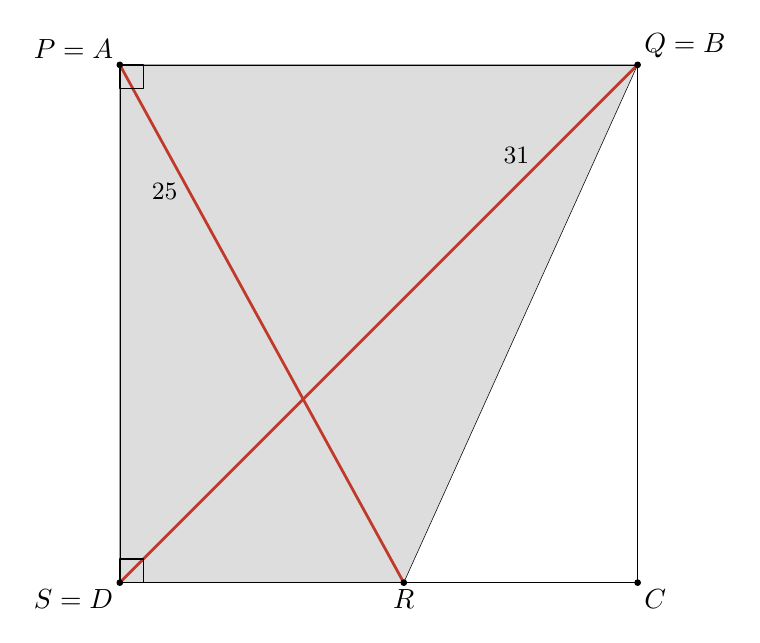
\begin{tikzpicture}
%! let s = 31/sqrt(2)
\tkzDefPoint(0.0,6.5760931){A} %! A = (0, s)
\tkzDefPoint(6.5760931,6.5760931){B} %! B = (s, s)
\tkzDefPoint(6.5760931,0.0){C} %! C = (s, 0)
\tkzDefPoint(0.0,0.0){D} %! D = (0, 0)
\tkzDefPoint(3.6062446,0.0){R} %! R = (17/sqrt(2), 0)
%! fact dist(B, D) == 31
%! fact dist(A, R) == 25
%! fact on_segment(R, C, D)
%! fact area(A, B, R, D) == 372
%! fact parallel(A, B, D, R)
%! fact perp(A, D, D, R)
\tkzFillPolygon[color=figtint](A,B,R,D)
\tkzDrawPolygon(A,B,C,D)
\tkzDrawPolygon(A,B,R,D)
\tkzDrawSegments[key](A,R B,D)
\tkzMarkRightAngle[size=.3,mk](A,D,R)
\tkzMarkRightAngle[size=.3,mk](D,A,B)
\tkzDrawPoints(A,B,C,D,R)
\tkzLabelPoint[above left,lbl](A){$P=A$}
\tkzLabelPoint[above right,lbl](B){$Q=B$}
\tkzLabelPoint[below right,lbl](C){$C$}
\tkzLabelPoint[below left,lbl](D){$S=D$}
\tkzLabelPoint[below,lbl](R){$R$}
\tkzLabelSegment[below left,pos=.22,len](A,R){$25$}
\tkzLabelSegment[above left,pos=.2,len](B,D){$31$}
\end{tikzpicture}
\end{document}
